\subsection{Neural Networks training LSTM}

\subsubsection{Data preparation.}

LSTM neural networks are based on time series. Hence, we can only use the PEPSI dataset where the variable $day$ is present. The measurement sequences available in PEPSI goes from 145 days to a maximum of 595 days depending on the river. LSTM neural networks learn from a single river time series. Therefore, the time series we have are too small. We need to periodise the time series over several years to obtain a sufficiently large dataset and a pattern that repeats over the years. We assume that the river flow rate is the same over the years. Because of this size problem, we focus our study on the \textit{Missouri Downstream} river which has observations for 595 days. We first cut the time series around 360 days to have a full year. We also have to cut it at a day where the river discharge is close to the first day river discharge to have continuity between each year. Once this compromise has been found, we can periodise the time series of \textit{Missouri Downstream} river. 

\begin{figure}[H]
    \begin{subfigure}{0.45 \textwidth}
        \centering
        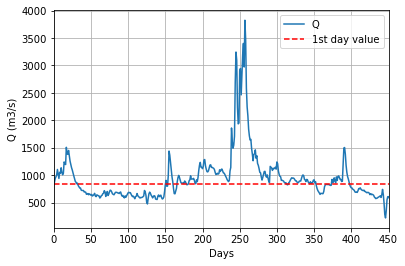
\includegraphics[scale = 0.5]{Graph/1year.png}
        \caption{Initial time series}
        \label{fig:my_label}
    \end{subfigure}
    \centering
     \begin{subfigure}{0.45 \textwidth}
         \centering
        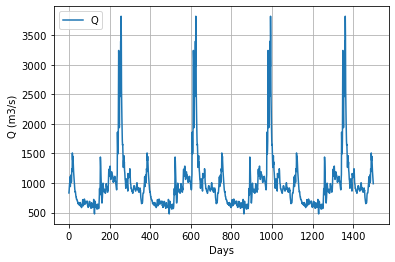
\includegraphics[scale = 0.5]{Graph/5years.png}
        \caption{5 years of river flow after the periodisation}
        \label{fig:periodisation}
     \end{subfigure}

  \caption{Periodisation of \textit{Missouri Downstream} river flow}
  \label{fig:period_Mis}
\end{figure}

 We periodise on $5$ years. Figure \ref{fig:period_Mis} shows the periodisation of the initial time series and then the new river discharge on 5 years.

\subsubsection{Architecture of the neural networks.}

We choose 80\% - 20\% for the proportion between the training and the testing set. We set the sequence length at 16, i.e. the number of days used to predict the next day, and the batch size also to 16. We change the features used for the learning phase. \textit{Flowacc} is now constant in the time series because we consider a single river and a single reach. Thus, we put \textit{W}, \textit{dA} and \textit{S} as input data, and \textit{Q} always as output data. \\

For \textit{Missouri Downstream} river, we obtain a training set composed of 2944 days, and 736 days for the testing set. We hence get 91 batches available for the training. We build a neural network with 10 LSTM cells which give us 571 trainable parameters. Mean Squared Error is set as the loss function and as a metric, and Mean Absolute Error and nRMSE as other metrics. Finally, we run the neural networks trough 20 \textit{epochs}. 

\subsubsection{Long Short-Term Memory Network training.}
We compute and display the metrics MAE and nRMSE through the $epochs$ (see Figure \ref{fig:metricsLSTM}). 
\begin{figure}[H]
    \begin{subfigure}{0.45 \textwidth}
        \centering
        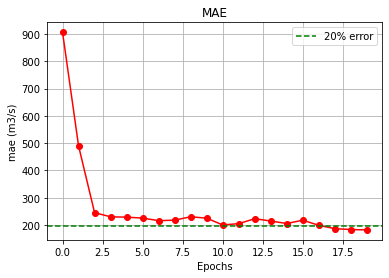
\includegraphics[scale = 0.5]{Graph/mae_lstm.png}
        \label{fig:my_label}
    \end{subfigure}
    \centering
     \begin{subfigure}{0.45 \textwidth}
         \centering
        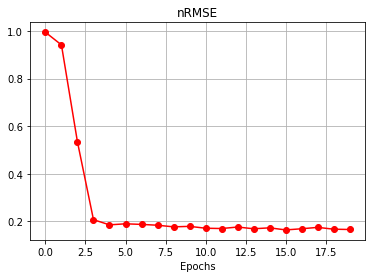
\includegraphics[scale = 0.5]{Graph/nrmse_lstm.png}
        \label{fig:my_label}
     \end{subfigure}
     \caption{Evolution of $MAE$ and $nRMSE$ during the learning phase}
     \label{fig:metricsLSTM}
     
\end{figure}

First, we note the steep and rapid decrease of both of the metrics and the beginning of their convergence from the fifth epoch. MAE converges slowly from the fifth epoch onwards and finally reaches the 20\% physical error rate. The nRMSE also decrease slowly from the fifth epoch under 
20\% of error. Each metrics converge stably to a satisfying rate.  

\subsubsection{Long Short-Term Memory Network testing.}

We compute now the river flow prediction computed on the testing test, and the solution of the Low-Froude model computed with the prediction given by the LSTM network. In table \ref{tab:perf_lstm}, we display the performance of each prediction with nRMSE.

\begin{figure}[H]

\centering
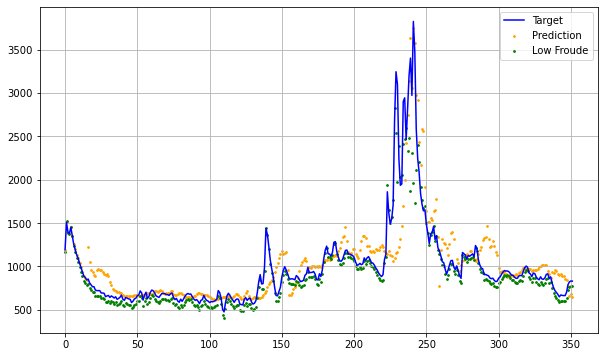
\includegraphics[scale = 0.5]{Graph/pred_low_fr_missour_lstm.png}
\caption{Prediction of $MissouriDownStream$ by LSTM and Low-Froude Model}
\label{fig: lest result} 
\end{figure}

\begin{table}[H]
    \centering
    \begin{tabular}{|c|c|}
    \hline 
        
         Q predicted & 0.28626674 \\
         \hline 
         Low-Froude model & 0.31700262 \\
    \hline
    \end{tabular}
    \caption{nRMSE Performance of the models}
    \label{tab:perf_lstm}
\end{table}

In Figure \ref{fig: lest result}, we observe 3 different hydrographs \textit{Missouri Downstream} river. Each one are close to each other. River discharge seems to be well estimated. The nRMSE of the prediction by LSTM network and the river flow rate computed by the Low-Froude model are around 30\% of error. The results obtained are hence satisfying. Only the prediction of the highest peak of river discharge observed around day 230, what we would expect to be a flood, appears to be less accurate than the smaller peaks. The low nRMSE of the solution of the Low-Froude model shows us that LSTM prediction is consistent with the Low-Froude model. 
We conclude that the architecture of LSTM enables to predict accurately discharge values for this river. The condition to obtain such results is to have enough data, and so to have enough days / years to train on. Hence, we see that a good solution is the duplication of an existing time series as we perform in our study.

\subsection{Discussion.}

As a conclusion, we computed two different neural networks, which have two different aims.

First, the Artificial Neural Network is a versatile neural network, as it can predict the river discharge on any river. But the quality of the prediction will depend nearly exclusively on the amount of data available : to be efficient, the ANN needs to train itself on a huge dataset in terms of size.

Second, the Long Short-Term Memory network is at the opposite of the Artificial Neural Network : it does not need a huge amount of data, as 5 years of data from a river are sufficient, which represents a small dataset size. However, the network can just predict the river discharge of a particular river, which can be restrictive.\newline

Thus, the common and crucial point is the following : to be efficient, the two neural networks need an important amount of data. In this way, the SWOT mission seems to be perfectly adapted, as it will collect many river data around the world.\newline

We will finish by mentioning the following point. During this study, we discriminated our rivers according to their river discharges. But actually, we will not possess this information about the new rivers we will want to predict the river discharge. Thus, separate the rivers according to other criteria, such as the flow accumulation or the width, could be a solution. A more precise discrimination could even be to separate the data according to river reaches, and not just on entire rivers.